
\documentclass[MASTER.tex]{subfiles} 
\begin{document} 
		\begin{frame}[fragile]
		\frametitle{dplyr : Grammar of data manipulation}
		\Large
		\textbf{What is dplyr?}
		\begin{itemize}
			\item dplyr is mainly authored by Hadley Wickham and Romain Francois. It is designed to be intuitive and easy to learn, thereby making ``doing things" in \texttt{R} more user-friendly.
			\item dplyr is a new package which provides a set of tools for efficiently manipulating datasets in \texttt{R}.
			\item dplyr is the next iteration of plyr, focussing on only data frames. \item dplyr is faster, has a more consistent API and should be easier to use. 
		\end{itemize}
	\end{frame}
		%==================================================================================== %
	\begin{frame}
		\frametitle{dplyr; Single Table Verbs}
		\Large
		dplyr aims to provide a function for each basic verb of data manipulating:
		\begin{itemize}
			\item \texttt{ filter() } (and \texttt{  slice() })
			\item \texttt{ arrange() }
			\item \texttt{ select() } (and \texttt{  rename() })
			\item \texttt{ distinct() }
			\item \texttt{ mutate() } (and \texttt{  transmute() })
			\item \texttt{ summarise() }
			\item \texttt{ sample\_n() } and \texttt{  sample\_frac() }
		\end{itemize}
		%	\begin{figure}
		%\centering
		%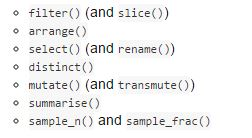
\includegraphics[width=0.7\linewidth]{images/singletableverbs}
		%
		%\end{figure}
	\end{frame}
	\end{document}